%% -------------------------------------------------------
% Preamable ---------------------------------------------
%--------------------------------------------------------
\documentclass[letter,12pt]{article}
%-------------------------------------------------------
%\usepackage [colorlinks, linkcolor=blue,
% citecolor=magenta, urlcolor=cyan]{hyperref}   % pdf links
\usepackage {hyperref}
\usepackage{tgtermes}
\usepackage[parfill]{parskip}
\usepackage{graphicx} % inserting image
\usepackage{setspace} % double/single spacing
\usepackage[top=2cm,right=2cm,bottom=2cm,left=2cm]{geometry} % margins 
\usepackage{amsmath}  %math formulas
\usepackage{array}    %beautiful tables
\usepackage[export]{adjustbox} %aligning images
\usepackage{algorithm}
\usepackage{algorithmic}
\usepackage{color,soul} %highlight
\usepackage{subcaption}        %figures with subfigures
\usepackage{amssymb}         %fonts for N, R, ...

\graphicspath{{img/}} %where the images are

\newenvironment{tight_itemize}{
\begin{itemize}
  \setlength{\itemsep}{0pt}
  \setlength{\parskip}{0pt}
}{\end{itemize}}

\newenvironment{tight_enumerate}{
\begin{enumerate}
  \setlength{\itemsep}{0pt}
  \setlength{\parskip}{0pt}
}{\end{enumerate}}


\newcommand*\rfrac[2]{{}^{#1}\!/_{#2}}
\newcommand*{\hvec}[1]{\mathbf{#1}}
\newcommand*{\hmat}[1]{\mathbf{#1}}

% -------------------------------------------------------
% Author and title---------------------------------------
%--------------------------------------------------------
\title{Generation of Boundary Conforming Three-dimensional Anisotropic Meshes}
\date{April 2016} 
\author{Shayan Hoshyari}

% -------------------------------------------------------
% Begin document-----------------------------------------
%--------------------------------------------------------
\begin{document}
\maketitle
\tableofcontents
\pagenumbering{arabic}

% -------------------------------------------------------
% -------------------------------------------------------
% Intro      --------------------------------------------
%--------------------------------------------------------
% -------------------------------------------------------

\section{Introduction}

High-order accurate methods for simulation of fluid flow problems, are
among the highly pursued research frameworks in Computational Fluid
Dynamics, due to their potential to reduce the computational effort
required for a given level of solution accuracy. My
current thesis project is to generalize our in house high order
turbulent viscous flow finite volume solver\cite{jalali} to handle
three dimensional geometries.

Conventional mesh generators create linear cells near the curved
boundaries. However, high order numerical methods must account for the
curved boundary in order to maintain their order of accuracy. For an
isotropic mesh curving the faces on the boundary is sufficient. On the
other hand, for anisotropic meshes, which are common in turbulent flow
simulations, the mesh deformation should be propagated inside the
domain to prevent unacceptable self intersecting elements.

To convert a three-dimensional anisotropic linear element mesh to a
boundary conforming curved mesh, a solid mechanics analogy is
used. The initial linear mesh is modeled as an elastic solid. When the
boundary of the solid is deformed to match the curved boundary, the
internal deformation of the solid will create the desired conforming
curved mesh.

The equations modeling the elastic solid, i.e. Navier Equations, are 
written as\cite{lai}:
%
\begin{equation}
\label{eq:ela-1}
\nabla \cdot \sigma = 0
\end{equation}
%
Where $\sigma$ is the symmetric three dimensional stress tensor and
related to the displacement vector through the formulas :
%
\begin{align*}
& \sigma_{11} = (2 \mu + \lambda) u_x + \lambda v_y +  \lambda w_z \\
& \sigma_{22} = \lambda u_x + (2 \mu + \lambda) v_y +  \lambda w_z \\
& \sigma_{33} = \lambda u_x + \lambda v_y +  (2 \mu + \lambda) w_z \\
& \sigma_{12} = \mu u_y + \mu v_x \\
& \sigma_{13} = \mu u_z + \mu w_x \\
& \sigma_{23} = \mu v_z + \mu w_y
\end{align*}
%
Where $u$, $v$ and $w$ denote the components of the displacement
vector, $\mu$ and $\lambda$ are the Lame's coefficients, and the
subscripts denote partial differentiation. The Lame's coefficients are
among the properties of the solid, and will be considered constant
throughout the domain.

This project deals with the solution of the system of equations
\eqref{eq:ela-1} using the finite element method, as a starting step for
a code that can convert linear mixed element three-dimensional meshes
into curved boundary conforming ones.  Based on our current
two-dimensional mesh curving code we know that the Galerkin Method
with $C_0$ cubic polynomial basis functions is a suitable approach to
solve this system of equations, and that affine mappings will work for
all the mesh elements, as the boundary of the initial domain is the
actual linear mesh.

The libMesh\cite{kirk} Library is used to implement the numerical
method. libMesh is a C++ library that facilitates the implementation
of many finite element methods in parallel. Internally, this library
uses PETSc\cite{balay} to solve the large linear system of equations
arising from discretizing the equations.

% -------------------------------------------------------
% -------------------------------------------------------
% Numerical Method  -------------------------------------
%--------------------------------------------------------
% -------------------------------------------------------
\section{Numerical Method}

The numerical method is constituted of two main parts, i.e., weak
formulation of the problem, and the boundary conditions. Other parts,
such as defining the basis functions, are automatically handled by the
software library, and we only have to make the correct choice.

% -------------------------------------------------------
%                     weak formulation
% -------------------------------------------------------
\subsection*{Discretized Weak Formulation}

We are interested in the weak formulation of the system
\eqref{eq:ela-1} with boundary conditions in the form:
%
\begin{equation}
\label{eq:bdry-1}
\hmat{\sigma} \hat{n} + \hmat{Q}(x) \hvec{u} = \hvec{t}(x)
\end{equation}
% 
Where $\hat{n}$ is the unit normal, the vector $\hvec{t}$ and the
matrix $\hvec{Q}$ are only functions of spacial coordinates, and
$\hvec{u}$ is the displacement vector, i.e., $\hvec{u} = (u,v,w)$. We
will show that both the Dirichlet and Neumann boundary conditions can
be implemented in this form.

% ------------------------ Reformulation
The first step is to recast equation \eqref{eq:ela-1} into the
following more convenient form:
%
\begin{equation}
  \begin{aligned}
    \label{eq:ela-2}
    &-\nabla \cdot \left[
      \hmat{K_{11}} \nabla u + 
      \hmat{K_{12}} \nabla v + 
      \hmat{K_{13}} \nabla w  
      \right]  = f_1
    \\
    &-\nabla \cdot \left[
      \hmat{K_{21}} \nabla u + 
      \hmat{K_{22}} \nabla v + 
      \hmat{K_{23}} \nabla w  
      \right]  = f_2
    \\
    &-\nabla \cdot \left[
      \hmat{K_{31}} \nabla u + 
      \hmat{K_{32}} \nabla v + 
      \hmat{K_{33}} \nabla w  
      \right]  = f_3
  \end{aligned}
\end{equation}
%
The functions $f_i$ are identically zero except when a manufactured
solution is used. The fourth order tensor $\hmat{K}$ is defined as 
\[
K_{ijkl} = \lambda \delta_{ik} \delta_{jl} + 
\mu ( \delta_{ij}\delta_{kl} + \delta_{il}\delta_{jk} )
\]
%
Where $\delta_{ij}$ is the Kronecker delta.

% ------------------------ Finding the weak form

Now multiplying the first equation by a test function $\phi_i$,
integrating over the domain, and using the approximations $V=\sum_j
U_j\phi_j$, $V=\sum_j V_j\phi_j$,and $W=\sum_j W_j\phi_j$ we will get the
desired weak form.

\begin{equation}
  \begin{aligned}
      %
    & \sum_j U_j 
    \left( 
    \int_\Omega \nabla \phi_i \cdot \hmat{K}_{11} \nabla \phi_j +
    \int_{\partial \Omega} Q_{11} \phi_i \phi_j
    \right) +
    %
    \\ &\sum_j  V_j
    \left( 
    \int_\Omega \nabla \phi_i \cdot \hmat{K}_{12} \nabla \phi_j +
    \int_{\partial \Omega} Q_{12} \phi_i \phi_j
    \right) +
    %
    \\ &\sum_j  W_j
    \left( 
    \int_\Omega \nabla \phi_i \cdot \hmat{K}_{13} \nabla \phi_j +
    \int_{\partial \Omega} Q_{13} \phi_i \phi_j
    \right) 
    %     
    \\ 
    &= \int_\Omega f_1 \phi_i + 
    \int_{\partial \Omega} t_1 \phi_i
    %
  \end{aligned}
\end{equation}

The weak form of the second and third equations can also be found
similarly, to form a linear system of equations $\hmat{A} \hvec{U} =
\hvec{b}$.

% -------------------------------------------------------
%                      boundary conditions
% -------------------------------------------------------
\subsection*{Boundary Conditions}

We are mostly interested in imposing the Dirichlet boundary condition
on our boundaries to enforce the curved boundary conformity. We use
the penalty method\cite{oden} for this job. In the penalty method the
Dirichlet boundary condition is replaced by:
\[
\hmat{\sigma} \hat{n} + \beta \hmat{I} \hvec{u} = \beta \hvec{u}_D(x)
\]
Which is equal to setting $\hmat{Q}=\beta \hmat{I}$ and $\hvec{t} =
\hvec{u}_D(x)$. Where $\beta$ is a huge number in the order of
$10^{10}$. Because of the machine rounding off errors, this condition
will have the same result as directly enforcing
$\hvec{u}=\hvec{u}_D(x)$. This method is especially convenient when
basis functions other than Lagrange are used, where each degree of
freedom will not necessarily correspond to the solution value at a
certain point.

In other cases we might want to let the boundary move freely. This can
be achieved by setting $\hmat{Q}$ and $\hvec{t}$ equal to zero.

% -------------------------------------------------------
%                      boundary conditions
% -------------------------------------------------------
\subsection*{Finishing Touches}

After experimenting with the libraries' different options the following choices
were made to be used in the solver code:

\begin{itemize}

\item The Lame' coefficients are found from the relations $\mu = E /
  (2 (1+\nu))$ and $\lambda = (\nu E)/((1+\nu)(1-2 \nu))$. $\nu$ is
  the Poisson's ratio, which is set to be 0.3. Due to our boundary
  conditions the Young's modulus, $E$ cancels out of the equations (except
  for the manufactured solution case) so we simply choose the value of
  $1$ for it.

\item All the integrals are evaluated using the Gauss Quadrature
  formula of order $2p+1$ where $p$ is the order of basis function
  polynomials.

\item The linear system of equations is solved using the Conjugate
  Gradient method preconditioned with block ILU(2). It should be
  mentioned that PETSc's default matrix reordering method fails when
  cubic basis functions are used and a different method, e.g. the
  Reverse Cuthill-McKee (RCM), has to be used.

\item libMesh supports three families of $C_0$ polynomials in three
  dimensions. Lagrange, Hierarchic\cite{zien} and
  Bernstein\cite{far}. While all three expand the same function space,
  there are limitations in terms of library support. Also the
  stiffness of the linear system is different for each family. We will
  study this phenomenon in the results section.

\item For simplicity all the problems will be solved using hexahedral
  meshes. When using quadratic basis functions the code can work with
  other element shapes as well. Cubic basis functions, on the other
  hand, are only supported for hexahedra in libMesh.

\end{itemize}

% -------------------------------------------------------
% -------------------------------------------------------
% Results      ------------------------------------------
%--------------------------------------------------------
% -------------------------------------------------------

\section{Results}

The results are chosen slightly different from the project
proposal. In the warm up stage the equations are solved in a simple
box geometry and the accuracy is verified using a manufactured
solution. In part A a real problem is solved and a linear mesh is
actually curved. However, the geometry is simple which enables simple
projection of points from the linear mesh boundary to the actual
curved boundary. The geometry selected in Part B is chosen to mimic an
actual three dimensional airfoil. Unlike the last part, projection of
points onto the boundary is challenging and requires solving a
nonlinear system of equations.

% -------------------------------------------------------
%                            MMS
% -------------------------------------------------------
\subsection*{Manufactured solution in a box}

A manufactured solution will be used to verify the accuracy of the
implemented method. The geometry is a cube with unit sides while
Dirichlet boundary conditions will be imposed on all the boundaries.
The manufactured solution has the following form \footnote{I should
  confess that this is a poor choice for the manufactured solution
  especially due to the term $\sinh(2\pi z)$. This causes the solution
  to be too big at certain regions. $\cos(\sinh(z))$ would have been a
  better candidate. }:
%
\begin{align*}
& u = \cos(\pi x) \cos(\pi y) \cosh(\pi z) \\
& v = \cos(\pi x) \cos(2 \pi y) \cosh(\pi z) \\
& w = \cos(2 \pi x) \cos(\pi y) \cosh(2 \pi z) 
\end{align*}
%
The source terms $f_i$ are subsequently calculated from equation
\eqref{eq:ela-2} with the aid of maple. 

The equations are solved on a series of refined meshes comprised of 5,
10 and 20 elements in each direction. Figure \ref{fig:box} shows the
behavior of error norms with respect to mesh refinement. As expected
the $H^1$ and $L_2$ norms are of order $p$ and $p+1$
respectively. Where $p$ is the order of basis function
polynomials. This verifies the correct implementation of the numerical
method and correct choice of quadrature accuracy. The results shown in
Figure \ref{fig:box} are obtained using Hierarchical basis functions.

\begin{figure}
  \centering
  \begin{subfigure}{0.65\textwidth}
    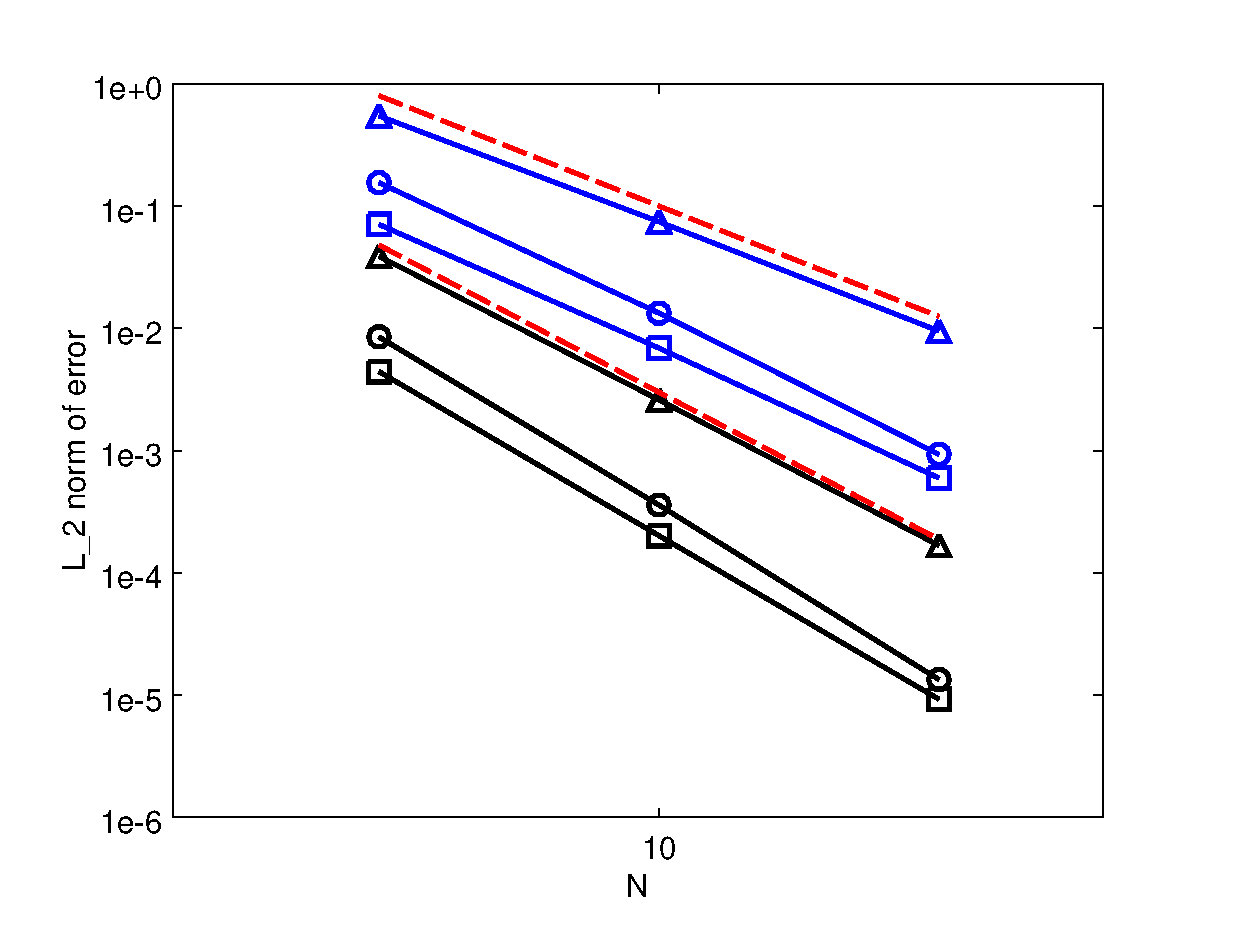
\includegraphics[width=.95\linewidth,center]{box-l2.eps}
  \end{subfigure}
  % 
  \begin{subfigure}{0.65\textwidth}
    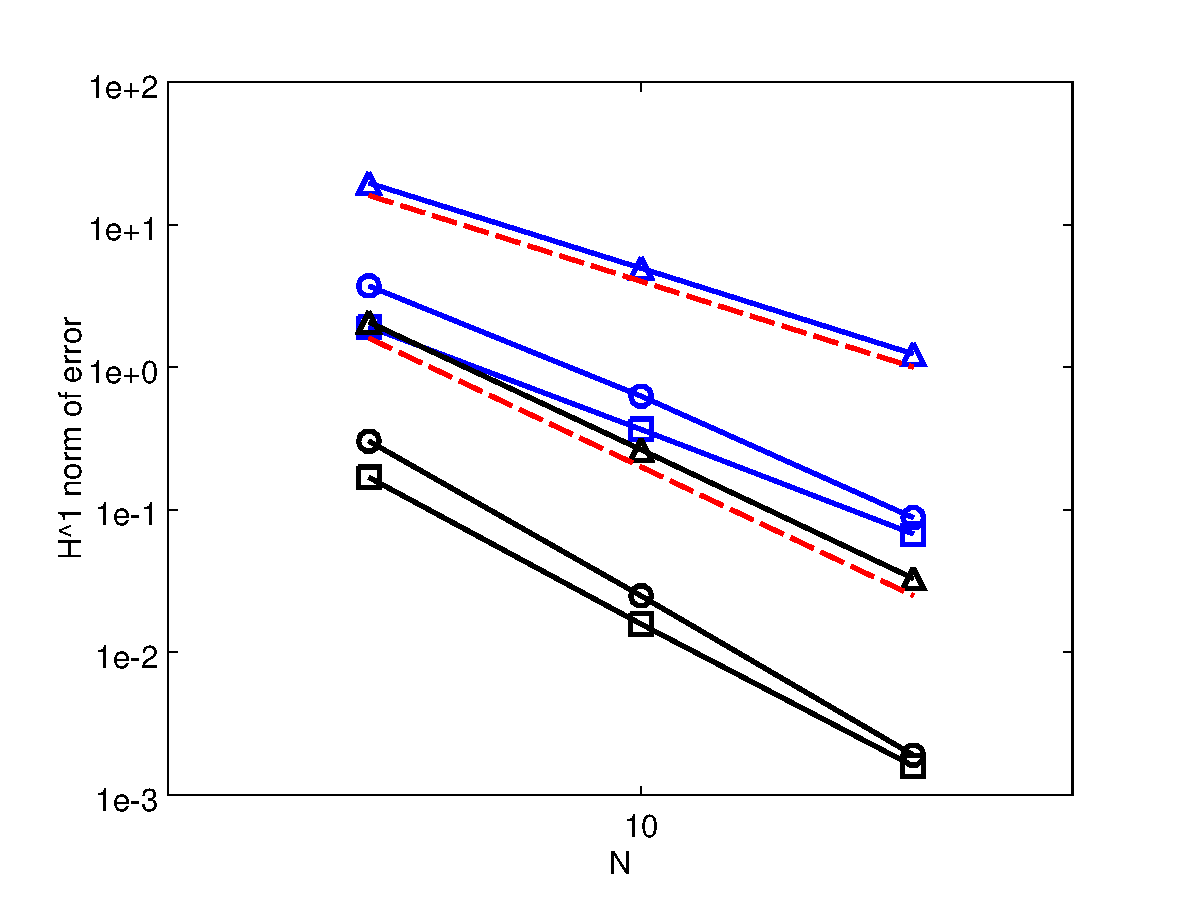
\includegraphics[width=.95\linewidth,center]{box-h1.eps}
  \end{subfigure}
  % 
  \caption{Norms of the error for the manufactured solution in a cubic
    domain. The blue lines are obtained by using quadratic basis
    functions while the black lines correspond to cubic basis
    functions. Triangles, Circles and Squares represent the error in
    $u$, $v$ and $w$ respectively. In the upper figure the red lines
    show third and fourth order reduction, whereas in the lower figure
    they represent second and third order reduction.}
  \label{fig:box}
\end{figure}

% -------------------------------------------------------
%                            PART A
% -------------------------------------------------------
\subsection*{Curving an incomplete sphere mesh}

The geometry of this problem is a wedge with inner and outer radii of
$1$ and $2$ and arch length of $\pi/3$ revolved around the $z$ axis which
crosses the circle center and is perpendicular to one of the sides.
The geometry and some parts of the initial linear mesh are shown in
Figure \ref{fig:sphere-mesh}.

In this problem we are only interested in conforming the inner surface
of the incomplete sphere to the actual boundary. For any point on this
surface we impose a Dirichlet boundary condition in the form of:
\[
\hvec{U}_D(x) = \frac{\hvec{x}}{|\hvec{x}|} - \hvec{x}
\]
Which will ensure that every point on the surface of the linear mesh
will be moved to its projection on the original curved surface.  The
outer curved surface is held fix, i.e., $\hvec{U}_D(x)=0$. This is
aimed to be an imitation of the far field boundary in an actual
aerodynamic problem. Natural boundary conditions are imposed on the
other boundaries (sides).

The displacement field obtained using quadratic Lagrange basis
functions is shown in Figure \ref{fig:sphere-u}. As expected the
vertices of the original mesh are displaced only by a negligible
amount (due to the penalty method for boundary conditions), while the
midpoints of the elements are displaced the most. As we move in the
radial direction towards the outer surface the displacement gets
smaller and smaller as desired. Remember that we wanted the outer
surface to stay intact.

We are also interested to study how the basis functions can affect the
stiffness of the linear system and the convergence history. Figure
\ref{fig:sphere-conv} shows the convergence history for each case. It
appears that the Bernstein polynomials create a much better
conditioned system compared to the Hierarchic polynomials. Lagrange
polynomials also perform well. However, their cubic version is not
implemented in libMesh.


\begin{figure}
  \centering
  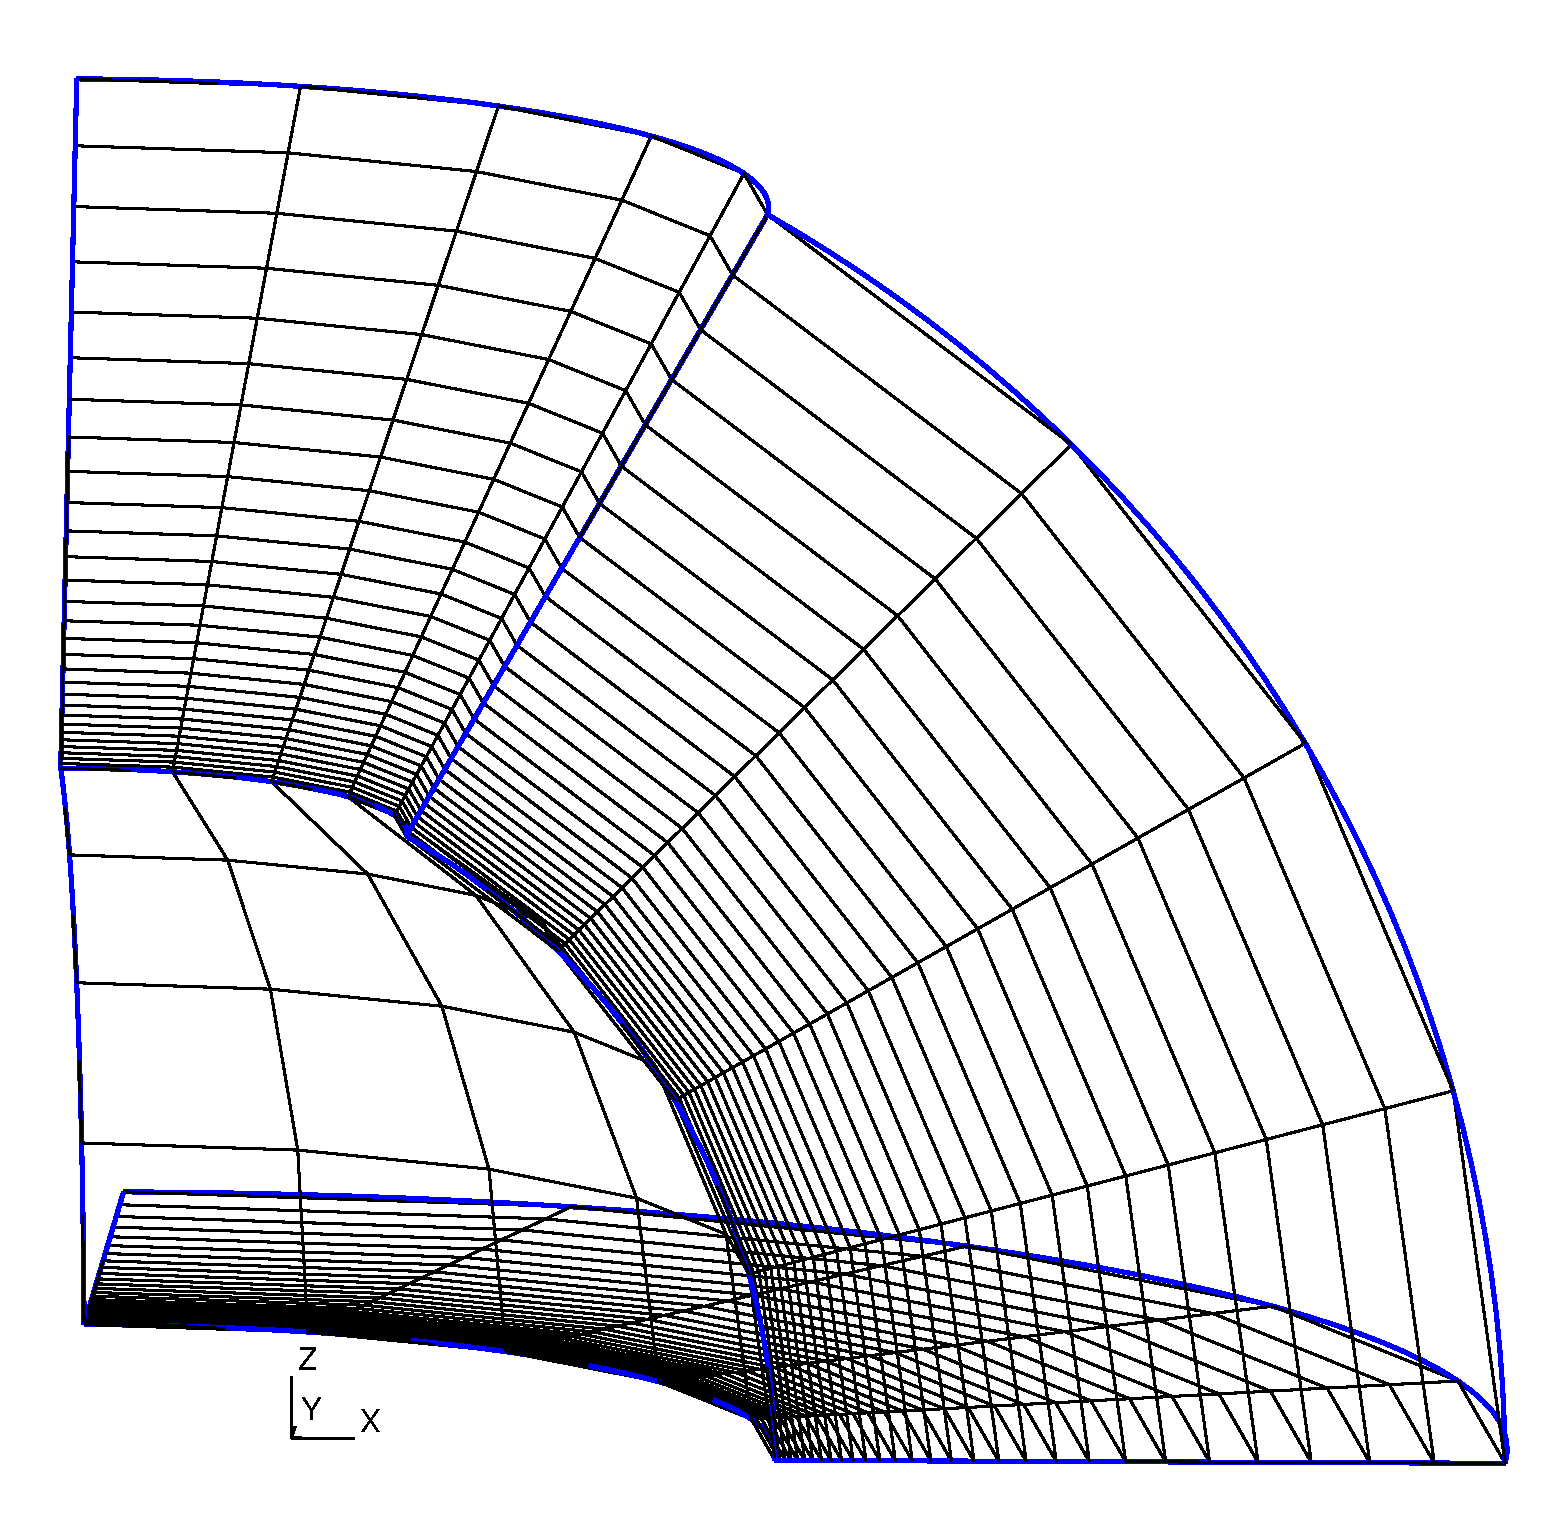
\includegraphics[width=.6\linewidth,center]{sphere-mesh.eps}
  \caption{Geometry and the mesh for the incomplete sphere problem.}
  \label{fig:sphere-mesh}
  %
  \vspace{0.5cm}
  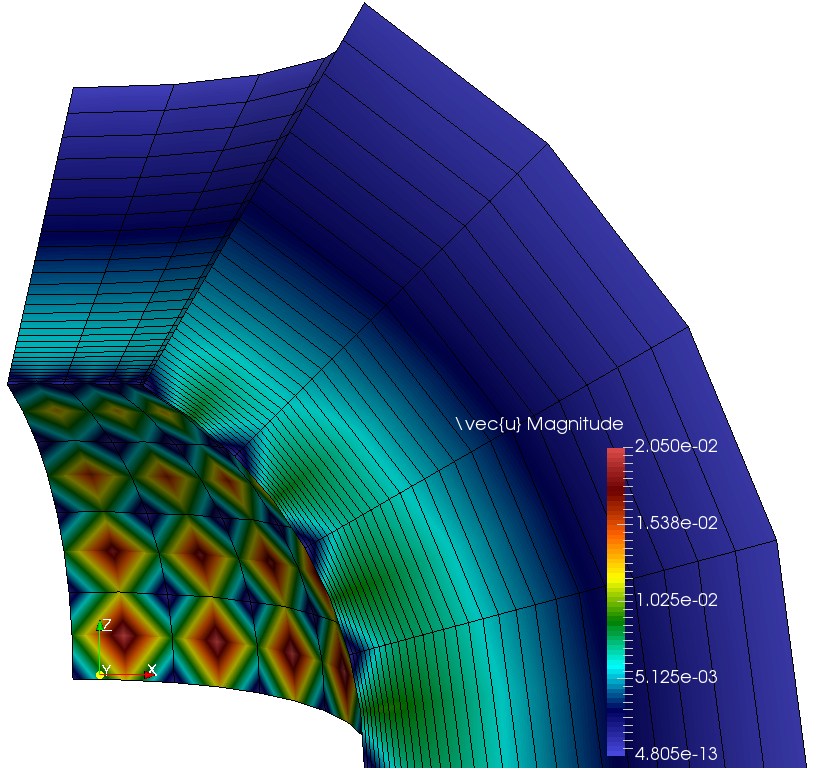
\includegraphics[width=.6\linewidth,center]{sphere-3d-2.png}
  \caption{The displacement magnitude for the incomplete sphere case.}
  \label{fig:sphere-u}
\end{figure}

\begin{figure}
  \centering
  \begin{subfigure}{0.65\textwidth}
    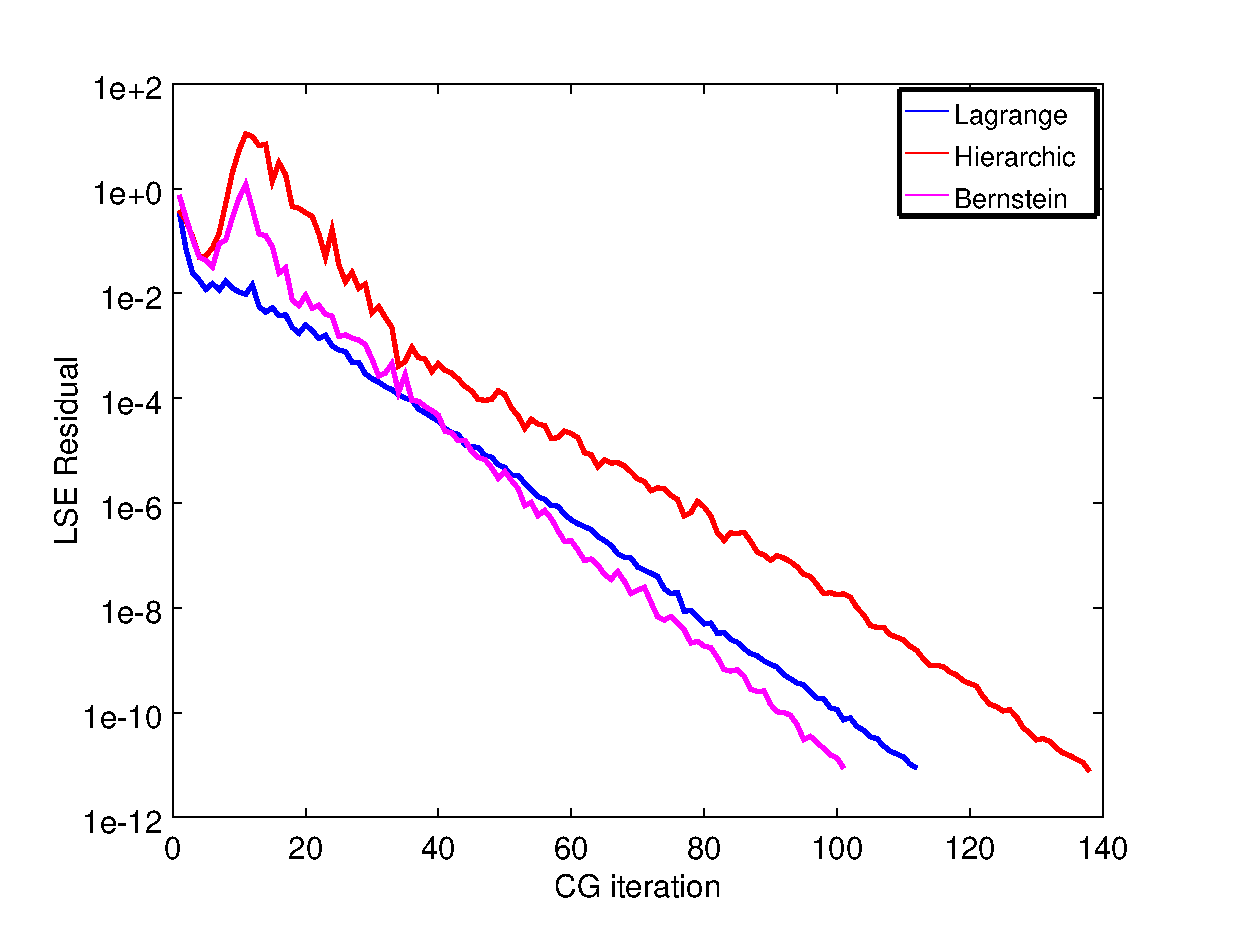
\includegraphics[width=.95\linewidth,center]{sphere-second-convergence.eps}
  \end{subfigure}
  % 
  \begin{subfigure}{0.65\textwidth}
    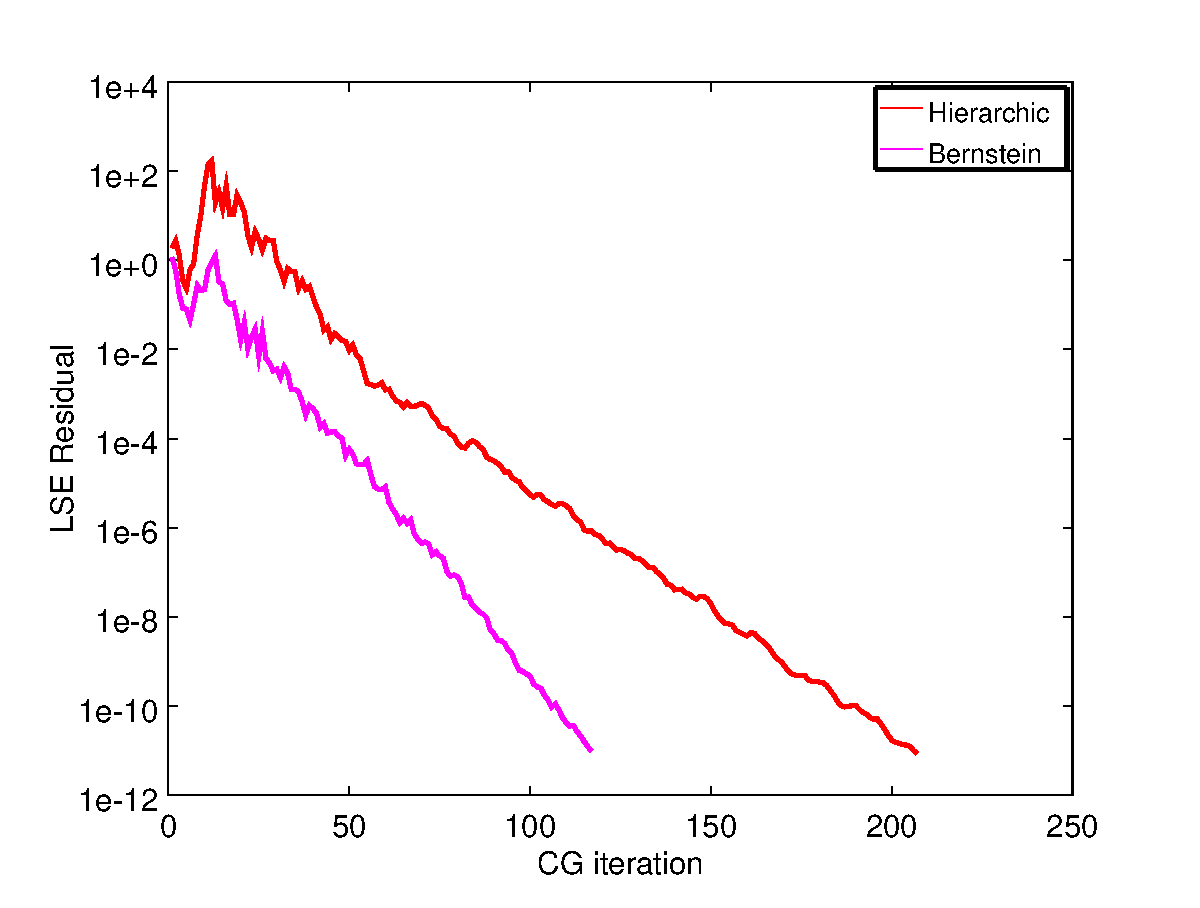
\includegraphics[width=.95\linewidth,center]{sphere-third-convergence.eps}
  \end{subfigure}
  %
  \caption{Convergence history for the incomplete sphere case. The upper and
    lower figures correspond to the quadratic and cubic basis
    functions respectively.}
  \label{fig:sphere-conv}
  %
\end{figure}

% -------------------------------------------------------
%                            PART B
% -------------------------------------------------------
\subsection*{Curving a three-dimensional airfoil mesh}

% -------------------------  boundary conditions
The geometry of this problem is shown in Figure
\ref{fig:bump-mesh}. The bump in the middle, a poor man's version of
an actual wing, is part of a circle which is extruded in the $4\hat{j}
+ \hat{i}$ direction and resized simultaneously.

We are interested in making the mesh conforming to the surface of the
airfoil. To do so we impose the following Dirichlet boundary condition on
the airfoil surface.
\[
\hvec{U}_D(\hvec{x}) = \text{Proj}(\hvec{x}) - \hvec{x}
\]
Where Proj$(\hvec{x})$ is the projection of the point $\hvec{x}$ onto
the airfoil surface, i.e., the line connecting $\hvec{x}$ and
Proj$(\hvec{x})$ is perpendicular to the airfoil surface.

To find Proj$(\hvec x)$ we first parametrize the airfoil
surface. Assuming $\hvec{y}$ is a point on the surface we shall have
\[
\hvec{y} = \hvec{y}(u,v)
\]
Subsequently the normal at $\hvec{y}$ is found to be
\[
\hat{n}(u,v) = \frac{\hvec{y}_u \times \hvec{y}_v}{|\hvec{y}_u \times
  \hvec{y}_v|}
\]
Now to find Proj$(\hvec{x}) = \hvec{y}$ we have to solve the following
non-linear system of equations for $u$, $v$ and $d$ (the
distance between $x$ and $y$):
\[
\hvec{x} - \hvec{y}(u,v) - d\hat{n}(u,v) = 0
\]
This equation is solved using PETSc's non-linear solver, which is a
combination of the Newton's method with finite difference Jacobian and
the line search method, for every surface quadrature point.

For this particular case the surface parametrization reads as:
\begin{align*}
  & \hvec{y}(u,v) = (u+(R_0 - bu)\sin(v), cu, (R_0 - bu)cos(v) -
  H_0(1-\frac{bu}{R_0})) \\
  %
  & 0<u<1.25, \qquad -\frac{\pi}{6}<v<\frac{\pi}{6} \\
  %
  & R_0=1, \qquad H_0=\cos(\frac{\pi}{6}), \qquad
  b=2, \qquad c=4
\end{align*}

For straight boundaries perpendicular to $y$ and $z$ axes the normal
displacement is enforced to be zero while natural boundary condition
is used for the tangent displacement. On the other hand, for the
straight boundaries perpendicular to $x$ axis free boundary condition
is used for all displacement components. I am suspicious that if
Dirichlet boundary conditions are used for all boundaries the system
of equations maybe be ill-posed. Intuitively, this can be explained by
the fact that the volume of the total solid cannot change arbitrarily.

% -------------------------  results

\begin{figure}
  \centering
  \includegraphics[width=.8\linewidth,center]{bump-mesh.eps}
  \caption{Geometry and the mesh for the airfoil problem.}
  \label{fig:bump-mesh}
\end{figure}

\begin{figure}
  \begin{subfigure}{0.9\textwidth}
  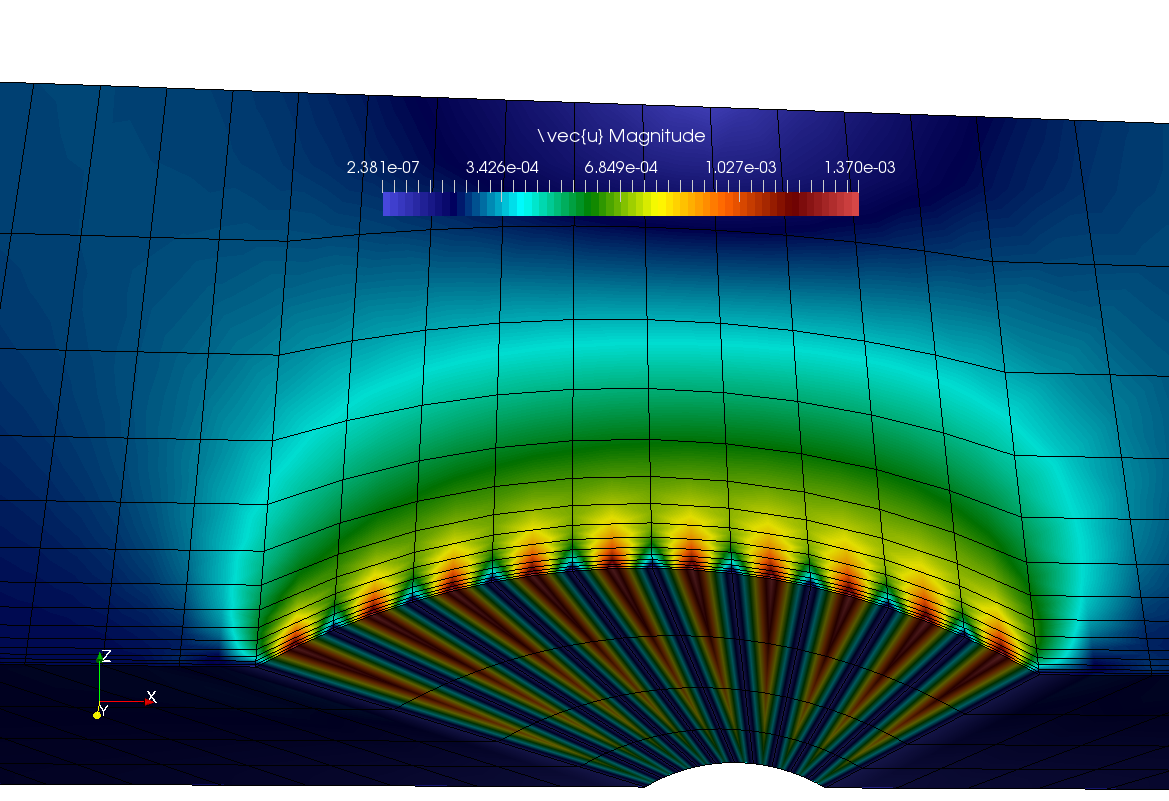
\includegraphics[width=.9\linewidth, center]{bump-front-3d.png}
  \caption{Front view.}
  \end{subfigure}
  %
  \begin{subfigure}{0.9\textwidth}
  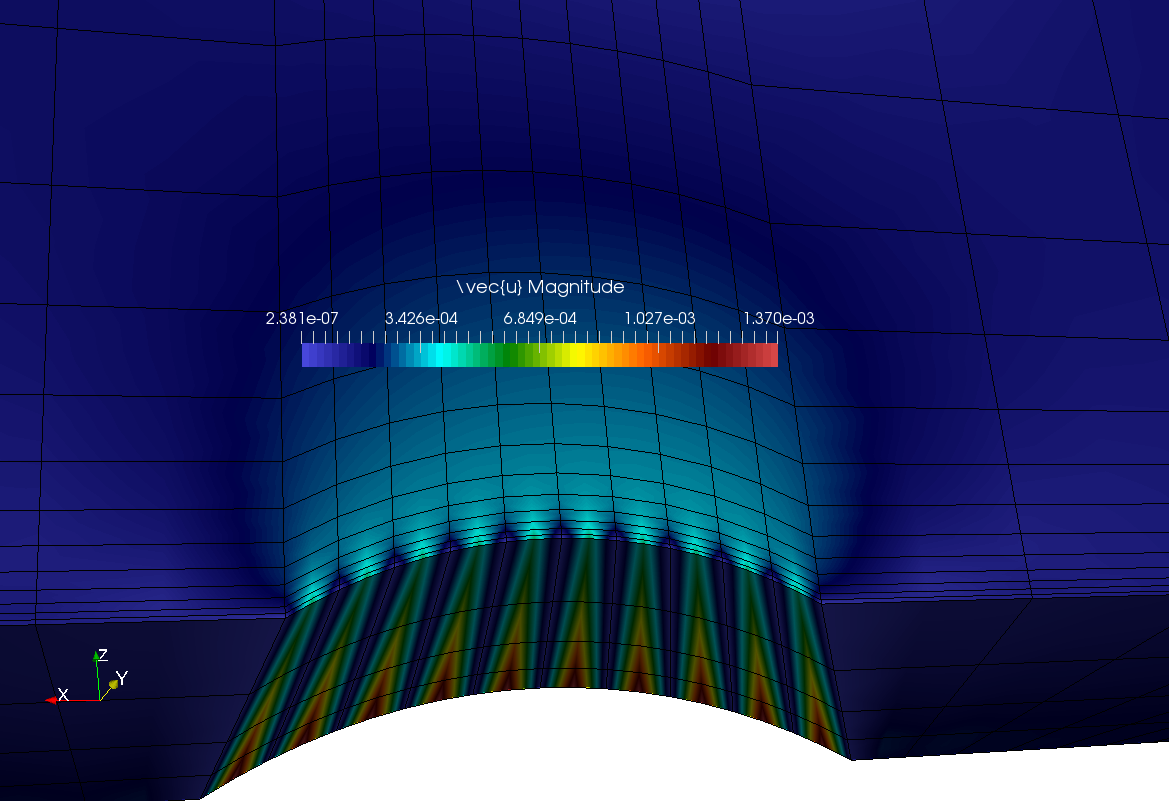
\includegraphics[width=.9\linewidth, center]{bump-back-3d.png}
  \caption{Back view.}
  \end{subfigure}
  %
  \caption{The displacement field for the airfoil case. }
  \label{fig:bump-u}
\end{figure}

\begin{figure}
  \centering
  \begin{subfigure}{0.65\textwidth}
    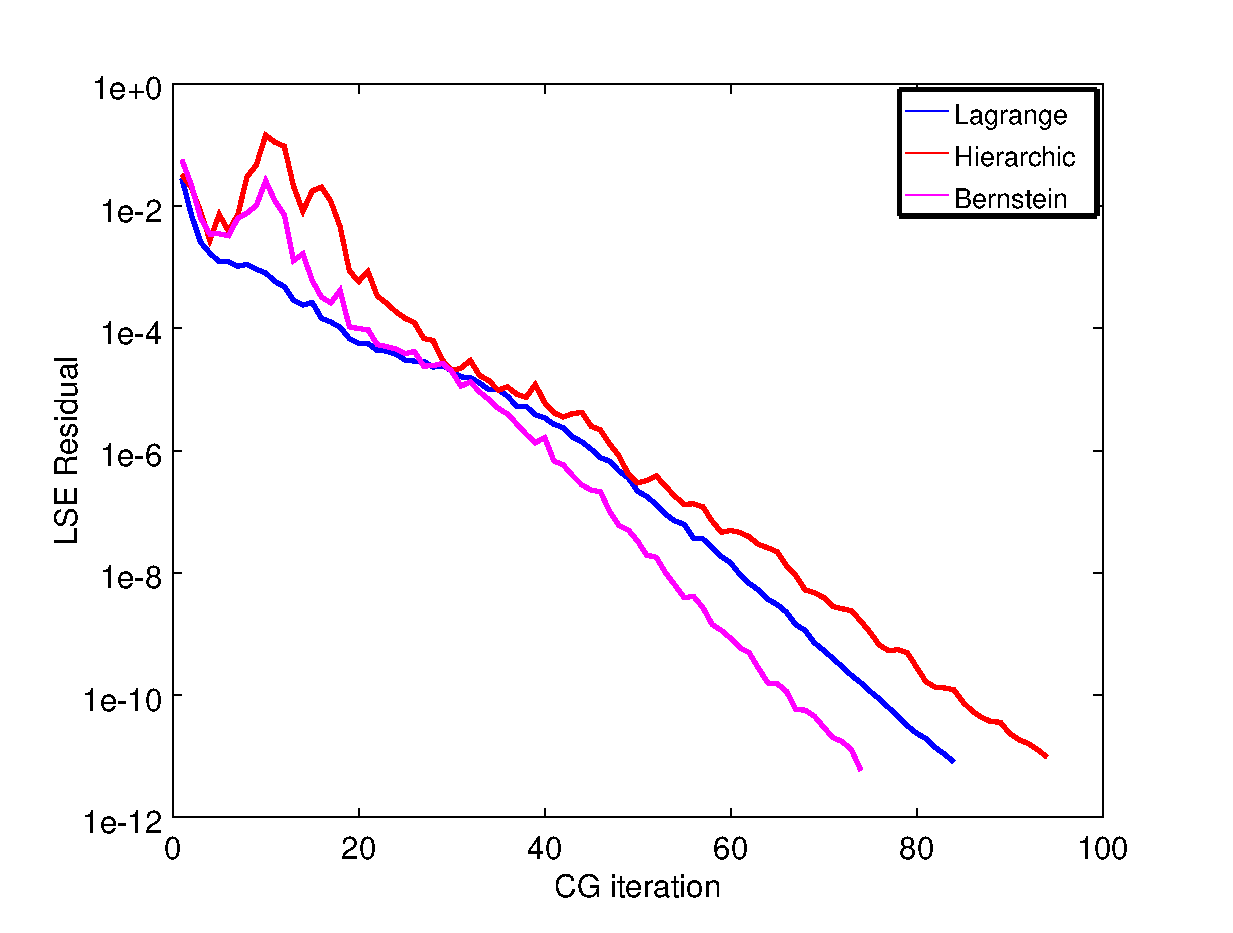
\includegraphics[width=.95\linewidth,center]{bump-second-convergence.eps}
  \end{subfigure}
  % 
  \begin{subfigure}{0.65\textwidth}
    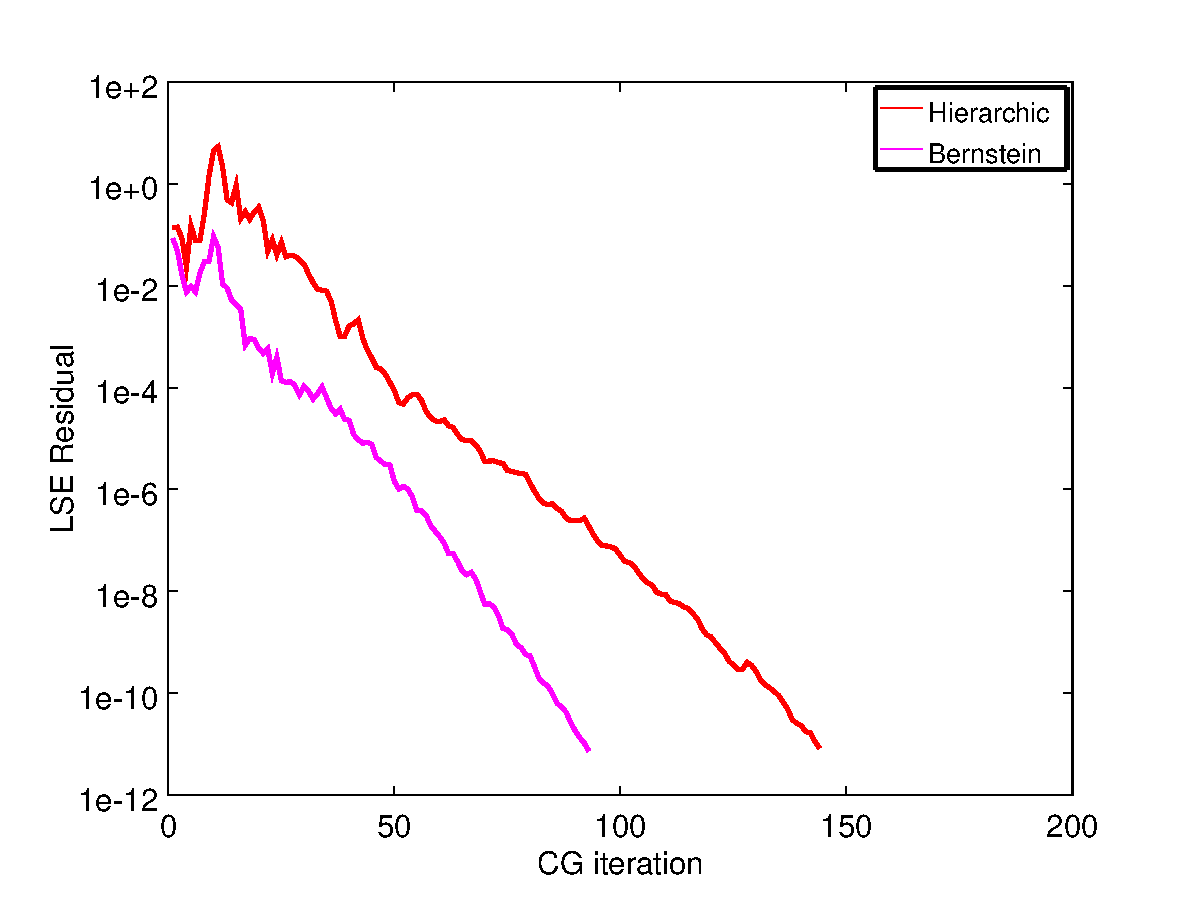
\includegraphics[width=.95\linewidth,center]{bump-third-convergence.eps}
  \end{subfigure}
  %
  \caption{Convergence history for the airfoil case. The top and
    bottom figures correspond to the quadratic and cubic basis
    functions respectively.}
  \label{fig:bump-conv}
  %
\end{figure}

Figure \ref{fig:bump-conv} shows the convergence history obtained by
using different basis functions. Bernstein polynomials outperform
their counterparts in this case as well. It is also noteworthy to
mention that the residual tends to increase in the initial iterations
except for Lagrange polynomials.

Figure \ref{fig:bump-u} shows the displacement field obtained using
quadratic Lagrange basis functions. Similar to the previous example
problem the vertices of the original mesh are displaced negligibly,
while the midpoints of the elements are displaced the most. The
displacement is propagated throughout the mesh, and tends to zero in
the midway to the top and side surfaces.

% -------------------------------------------------------
% bibliography-------------------------------------------
%--------------------------------------------------------
\bibliography{proposal}{} 
\bibliographystyle{plain}

\end{document}

